\documentclass[10pt,a4paper]{article}
\usepackage[utf8]{inputenc}
\usepackage[a4paper,margin=2.3cm]{geometry}
\usepackage{booktabs}
\usepackage{graphicx}
\usepackage{amsmath,amssymb}
\usepackage[hidelinks]{hyperref}
\usepackage{enumitem}
\usepackage{caption}
\usepackage{float}
\captionsetup{font=small,labelfont=bf}
\setlist{itemsep=2pt,topsep=3pt}
\setlength{\parskip}{3pt}
\setlength{\emergencystretch}{4em}
% Repository URL: replace with the real GitHub repository before submitting.
\newcommand{\repourl}{\url{https://github.com/hugogzfz/bd-assignment1-matmul}}

\title{\textbf{Assignment 1: How Runtime and Memory Scale in the Basic Triple-Loop\\Matrix Multiplication in C, Java and Python}}
\author{Hugo Gonz\'alez Fern\'andez\\[2pt]
Big Data \,$\cdot$\, Bachelor’s Degree in Data Science and Engineering\\
Universidad de Las Palmas de Gran Canaria\\
Academic year 2026--2027 \,$\cdot$\, Individual Assignment 1}
\date{October 2026}

\begin{document}
\maketitle

\begin{abstract}
\noindent\textbf{Question.} How do the runtime and the memory use of the textbook $O(n^3)$ multiplication of $n\times n$ \texttt{float64}
matrices grow with $n$ in C, Java and Python? \textbf{Method.} Three implementations of the same i--j--k triple loop read identical, seeded input
files; only the multiplication kernel is timed (monotonic timers, warm-up and repeated samples, median and IQR); peak resident memory is recorded per process;
every result is validated against NumPy with an a-priori error bound and the three languages produce bit-identical output. Budgets were $300$\,s per multiplication and $4$\,GiB.
\textbf{Results.} Time grows as $\approx n^{3.2}$ for $n\le400$, and the cost per multiply--add increases for larger matrices (C $1.0$--$1.4\to6.8$\,ns, Java $1.6\to11.1$\,ns).
Python is $49$--$75\times$ slower than C and Java at $50\le n\le1000$. Java \texttt{double[n][n]} falls $2.2$--$4.3\times$ behind C beyond $n\approx1000$,
and a supplementary flat-array variant removes most of the gap; C shows $\approx1.8$--$1.9\times$ spikes at $n=512$ and $1024$. Memory follows array storage ($24$, $\approx22$ and $\approx121$ bytes per $n^2$)
plus a runtime baseline ($1.8$, $45.7$, $9.8$\,MiB). The largest feasible sizes were $3000$ (C), $2048$ (Java) and $1250$ (Python).
\textbf{Scope.} One virtual machine, one compiler/JVM/interpreter version each, 2--10 repetitions: the conclusions are valid for these settings only and are not a general ranking of languages.
\end{abstract}

\section{Introduction and objective}

Dense matrix multiplication is the standard microbenchmark for studying how a programming language
implementation turns the same algorithm into machine work. This study compares the \emph{textbook triple-loop}
algorithm, which performs $n^3$ multiply--add operations on $n\times n$ matrices, in three languages:
C (ahead-of-time compiled), Java (JIT-compiled on the JVM) and Python (CPython, interpreted).

\paragraph{Research question.} \emph{How do the runtime and the memory use of the basic $O(n^3)$ multiplication of
$n\times n$ \texttt{float64} matrices grow with $n$ in C, Java and Python, when the three programs use the same
inputs, the same loop order and the same arithmetic on one documented machine?}

\paragraph{Factor and outcomes.} The factor that changes is the matrix size $n$ (from $10$ up to the largest size
that fits the declared budgets); the outcomes are the time of one multiplication (kernel only) and the peak resident
memory of the process.

\paragraph{Hypotheses (predictions, stated before running the experiments).}
\begin{enumerate}
  \item[H1] In every language the time grows approximately as $n^3$ (log--log slope $\approx 3$), but the constant
        factor differs.
  \item[H2] The order of speed is C $\lesssim$ Java $\ll$ Python, with Python one to two orders of magnitude slower
        than the compiled languages, because of interpreter dispatch and boxed floating-point objects.
  \item[H3] The cost per multiply--add is not constant: once the matrix $B$, which is read by columns, no longer
        fits in a cache level, the cost per operation increases.
  \item[H4] Memory is dominated by array storage: about $24\,n^2$ bytes for C and Java ($3$ matrices $\times 8$ bytes), a
        much larger $\approx 120\,n^2$ bytes for Python (each element is an 8-byte pointer plus a separately allocated
        float object), plus a fixed runtime baseline that is largest for the JVM.
\end{enumerate}

\paragraph{Scope.} Conclusions are limited to the implementations, compiler and runtime settings, inputs and the
virtual machine described in Section~\ref{sec:env}. They are \emph{not} a general ranking of programming languages.
Language-specific optimisations (loop reordering, blocking, libraries) are deliberately excluded; they belong to
the later assignments.

\section{Background}

\paragraph{Algorithm.} For $C = AB$ with $A,B\in\mathbb{R}^{n\times n}$, $c_{ij}=\sum_{k=1}^{n}a_{ik}b_{kj}$. The
direct evaluation needs $n^3$ multiplications and $n^3-n^2$ additions, hence $\Theta(n^3)$ work \cite{clrs}. All
three programs use the loop order $i$--$j$--$k$ and accumulate each $c_{ij}$ in a scalar before storing it.

\paragraph{Memory access pattern.} With row-major storage the inner loop walks $a_{ik}$ along a row (unit stride) but
$b_{kj}$ down a column (stride $8n$ bytes). Once a column of $B$ touches more cache lines than the cache can
keep for the next value of $j$, every access to $B$ becomes a cache miss; for stride $8n$ with $n$ a power of two,
many addresses additionally map to the same cache sets \cite{drepper,hennessy}. This is why the cost per
multiply--add is expected to rise with $n$ even though the operation count is exactly cubic.

\paragraph{Execution models.} C code is compiled to machine code before running. Java bytecode starts interpreted
and is compiled by HotSpot's tiered JIT (C1, then C2), including on-stack replacement of hot loops; array accesses
keep bounds checks unless the JIT can remove them. CPython executes bytecode in an interpreter: every
\texttt{A[i][k]*B[k][j]} involves several bytecode dispatches, index operations and the allocation of a new
\texttt{float} object.

\paragraph{Floating-point error.} For a sum of $n$ products, any evaluation order gives
$|\hat c-c|\le\gamma_n\sum_k|a_{ik}b_{kj}|$ with $\gamma_n=nu/(1-nu)$ and $u=2^{-53}$ \cite{higham}. Because all
entries here are non-negative, $\sum_k|a_{ik}b_{kj}|=c$, so each implementation has relative error at most
$\gamma_n$, and two different evaluation orders differ by at most $2\gamma_n$ \cite{goldberg}. This bound is used as the
acceptance tolerance (Section~\ref{sec:correct}).

\paragraph{Benchmarking practice.} The protocol follows common recommendations: report central value and spread
over repeated runs, separate warm-up from steady state for JIT-compiled languages, state exactly what is timed
and report the environment \cite{georges,hoefler}.

\section{Methodology}

\subsection{Implementations}
\label{sec:impl}
\begin{itemize}
  \item \textbf{C} (\texttt{src/c/matmul.c}): one contiguous row-major block of $n^2$ \texttt{double} per matrix; the
        kernel is a separate non-inlined function so repetitions cannot be merged by the compiler.
  \item \textbf{Java} (\texttt{src/java/MatMul.java}): \texttt{double[n][n]}, i.e.\ $n$ separately allocated row
        arrays; kernel in its own static method.
  \item \textbf{Python} (\texttt{src/python/matmul.py}): list of $n$ lists of $n$ boxed \texttt{float}; pure Python
        loops, \emph{no} NumPy in the kernel.
\end{itemize}
The kernel is identical in structure in all three:
\texttt{s = 0.0; for k: s += A[i][k]*B[k][j]; C[i][j] = s}, for $i$, $j$ in this order. The scalar accumulator
differs slightly from a \texttt{C[i][j] += \dots} form: it keeps the same operation order (so the results are
bit-for-bit identical, see Section~\ref{sec:correct}) and avoids language-specific aliasing effects in the
comparison. Unavoidable differences are the storage layouts above and the runtime behaviour (JIT, interpreter,
boxing). No library multiplication is used by any implementation.

\subsection{Inputs}
Matrices $A$ and $B$ for each $n$ are generated once with NumPy's \texttt{default\_rng} (PCG64) seeded with
$[20261012, n, w]$ ($w=0$ for $A$, $w=1$ for $B$), uniform in $[0,1)$, and stored as raw little-endian binary64
files. All three programs read the \emph{same files}, so the logical inputs are identical and no cross-language
random generator is involved. SHA-256 digests of all files are stored in \texttt{data/manifest.json}.

\subsection{Environment}
\label{sec:env}
All measurements were taken on one machine, sequentially, with no other workload running (the driver only polled
the child process every $0.5$\,s). Table~\ref{tab:env} lists the environment. The machine is a virtual machine
(KVM) with $2$ vCPUs; the frequency governor is not visible and the processes were not pinned to a CPU. Each
kernel is single-threaded; the JVM may place its JIT and GC helper threads on the second vCPU. Thread counts used
by numerical libraries are not relevant because no library is used in the kernels (NumPy is only used for
generating inputs and checking results, \emph{outside} the measurements) \cite{numpy}.

\begin{table}[H]
\centering\small
\begin{tabular}{lp{10.5cm}}
\toprule
Item & Value \\
\midrule
CPU & Intel(R) Xeon(R) Processor @ 2.80GHz \\
Cores / logical CPUs & 2 physical (vCPU), 2 logical; 1 thread(s)/core \\
Caches & L1d 64 KiB (2 instances), L2 2 MiB (2 instances), L3 33 MiB (1 instance) \\
RAM & 8030 MiB, swap 0 MiB \\
Virtualisation & KVM (full) \\
OS / kernel & Ubuntu 24.04.5 LTS, Linux 6.18.44-fc-v114 \\
Python & CPython 3.13.16 (GCC 13.3.0) \\
Java & OpenJDK 21.0.12.1 (HotSpot 64-bit server VM); flags -XX:+UseSerialGC -Xms256m -Xmx4g (default tiered JIT: C1+C2) \\
C compiler & gcc (Ubuntu 13.3.0-6ubuntu2~24.04.1) 13.3.0; flags -O2 -std=c11 -ffp-contract=off  (no -march=native; no -ffast-math) \\
NumPy (reference only) & 2.5.3 \\
Threads in the kernel & 1 (single-threaded); no CPU pinning; frequency governor: not exposed (virtual machine) \\
\bottomrule
\end{tabular}

\caption{Hardware and software environment.}
\label{tab:env}
\end{table}

\subsection{Fixed settings}
Fixed in every comparison: algorithm and loop order, numeric type (binary64), inputs, single thread, one process
per configuration, monotonic timers, kernel-only timing. C is compiled with
\texttt{gcc -O2 -std=c11 -ffp-contract=off} (no \texttt{-march=native}, no \texttt{-ffast-math}): this forbids fused
multiply--add and re-association, so the arithmetic is the same as in Java and Python. Java runs on OpenJDK~21
with the default tiered JIT and \texttt{-XX:+UseSerialGC -Xms256m -Xmx4g}. Python is CPython~3.13 with the cyclic
garbage collector disabled inside the timed region (the kernel allocates only floats, which are not GC-tracked, so
this only removes a source of pauses). Different compiler options for C are explored in a \emph{separate}
supplementary experiment (Section~\ref{sec:cflags}).

\subsection{What the timer includes}
\label{sec:timer}
\textbf{Kernel only.} The timed region is the triple loop. Reading the inputs, allocating $C$, zero-initialising
$C$ (so its pages are touched before timing), computing the checksum and dumping the result are \emph{outside} the
timer. In Python the row lists of $C$ are created outside the timer; the float objects that hold the results are
created by the kernel and are therefore inside it. Timers: \texttt{clock\_gettime(CLOCK\_MONOTONIC)} (C),
\texttt{System.nanoTime()} (Java), \texttt{time.perf\_counter\_ns()} (Python). The result of every multiplication is
consumed: after each timed sample a checksum of $C$ (plain left-to-right sum in row-major order) is computed and
recorded, and the final $C$ is written to disk and verified.

\subsection{Repetition, warm-up and summary statistics}
Each configuration $(\text{language},n)$ runs in its own process with a number of \emph{warm-up} samples
(excluded from the statistics but kept in the raw data) followed by \emph{measured} samples. The numbers depend
on the estimated time of one multiplication $\hat t$: $\hat t\le 1$\,s: 3 warm-up, 10 measured; $\le30$\,s: 1 warm-up,
5 measured; $\le120$\,s: no warm-up, 3 measured; larger: no warm-up, 2 measured. Fewer repetitions for costly runs
are a compromise forced by the budget (a single Python multiplication at the largest sizes takes minutes); the
resulting spread is reported through min--max and IQR, and the number of repetitions is given for every
configuration (Table~\ref{tab:time}). When $\hat t<50$\,ms a batch of $m=\lceil 0.1\,\text{s}/\hat t\,\rceil$
multiplications is timed and divided by $m$, and the reported value is the \emph{time per multiplication}. Reported
statistics are the \textbf{median} and the \textbf{inter-quartile range} (IQR, $Q_3-Q_1$). The runs for different
languages are interleaved by size (for each $n$: C, Java, Python) so that slow drift of the machine affects all
languages alike.

\subsection{Budgets and limits}
\label{sec:budgets}
Declared before the large runs: a single timed sample must complete within \textbf{300\,s}; peak resident memory per
run must not exceed \textbf{4\,GiB}. A run that violates a limit is killed and recorded as a \emph{timeout} or
\emph{memory failure}, never given an invented time. The driver does not attempt sizes whose predicted time exceeds
three times the limit and stops enlarging $n$ for an implementation after its first failure. The \emph{largest
feasible} size (all repetitions completed, results validated) and the \emph{largest attempted} size are reported
separately (Table~\ref{tab:limits}). Planning aid: three binary64 $n\times n$ matrices need $24n^2$ bytes
(e.g.\ $\approx 0.4$\,GB at $n=4096$), so memory was not expected to bind before time did.

\subsection{Memory metric}
The primary metric is the \textbf{peak resident set size} of the whole process (\texttt{VmHWM} from
\texttt{/proc/self/status}, read by each program just before it exits and before the result is dumped), so it
includes the runtime itself (JVM, interpreter) and all matrices. The kernel's own accounting
(\texttt{ru\_maxrss} from \texttt{wait4}) is stored as a cross-check. RSS is not the same quantity as managed-heap use
or as the arithmetic estimate of array storage, and it is not comparable with them directly; the model
lines in Figure~\ref{fig:mem} are estimates of array storage added to the measured baseline of the smallest run.
\textbf{Limitations:} RSS counts pages actually resident (not reserved), includes loader/library pages, and has
granularity of one page; the Python process also needs transient buffers while loading rows.

\subsection{Correctness}
\label{sec:correct}
Before any benchmark, \texttt{scripts/test\_correctness.py} runs all three programs on small cases whose answers are
known (scalar, hand-computed $3\times3$, non-commutative $2\times2$, zero matrix, identity on both sides,
all-ones, small-integer matrices; \emph{exact} equality required, all intermediate values are integers below $2^{53}$,
so there is no overflow or rounding), and on random matrices against NumPy's \texttt{float64} product (tolerance
$2\gamma_n$ relative, derived in Section~2; absolute tolerance $0$ because every reference entry is positive). It also
requires the three languages to produce \emph{bit-for-bit identical} results. During the benchmark every run dumps
its final product and the driver checks it element-wise against NumPy with the same tolerance, plus the checksum
against the reference sum (tolerance $\gamma_{n^2+2n}$). NumPy/BLAS serves only as a trusted reference and is
not one of the implementations under study.

\subsection{Supplementary experiments (exploratory, kept separate)}
\label{sec:supp}
The following experiments were designed \emph{after} looking at the main results, to test explanations for
patterns seen there; they are therefore exploratory, they are reported separately, and they do not change the
controlled comparison above. All use the same driver, inputs, budgets and validation.
\begin{enumerate}
  \item \textbf{C optimisation level} (Section~\ref{sec:cflags}): the C program compiled with \texttt{-O0}, \texttt{-O1},
        \texttt{-O2}, \texttt{-O3} and \texttt{-O3 -march=native} (always with \texttt{-ffp-contract=off}) at
        $n\in\{512,1000,1024\}$.
  \item \textbf{Sizes around powers of two} (Section~\ref{sec:pow2}): $n\in\{496,504,512,520\}$ and
        $\{1016,1024,1032\}$ for C, Java, and the variant below.
  \item \textbf{Java with a flat array} (\texttt{src/java/MatMulFlat.java}): the same Java algorithm with each matrix
        stored as one row-major \texttt{double[n*n]} (the layout used by the C program), to test whether the
        jagged \texttt{double[n][n]} layout explains the Java--C gap. Sizes $n\in\{500,1000,1250,1500,2000\}$ and the
        power-of-two neighbourhoods. Correctness is checked by the driver on every run (same tolerance), not by
        the unit-test script.
  \item \textbf{Between-process variability} (Section~\ref{sec:procvar}): C and Java at $n=1024$ in six
        independent processes (the main run, the power-of-two run and four dedicated repeats).
\end{enumerate}

\section{Results}

All values are medians of the measured samples; values in parentheses are IQRs. Times are \emph{per
multiplication}, kernel only (Section~\ref{sec:timer}). The raw samples (including warm-up) are in
\texttt{results/raw\_measurements.csv}; per-run information is in \texttt{results/runs.csv}.

\subsection{Correctness}
All $52$ checks of the pre-benchmark test script passed (Table~\ref{tab:correct}); the maximum observed relative
error against NumPy was $7.6\times10^{-16}$ ($n=100$), far below the a-priori bound. In the benchmark, all
\textbf{92 completed runs} (43 of the main campaign and 49 supplementary) passed the element-wise check and the checksum
check (largest relative error $8.3\times10^{-15}$, i.e.\ below $10\,\%$ of the accepted bound; per-run values in
\texttt{runs.csv}), and the final $C$ of C, Java and Python was \textbf{bit-for-bit identical} for every size where
more than one language completed (SHA-256 of the dumped matrix, \texttt{results/summary\_bitwise.csv}). The
identical bits are expected because all three programs use the same operation order, binary64 arithmetic and no
fused multiply--add.

\begin{table}[H]
\centering\footnotesize
\begin{tabular}{llrrl}
\toprule
Test (all three languages) & Check & Max. rel./abs. error & Tolerance & Result \\
\midrule
scalar 1x1 (3*4) & exact & 0 & 0 (exact) & pass \\
hand-computed 3x3 & exact & 0 & 0 (exact) & pass \\
2x2 non-commutative & exact & 0 & 0 (exact) & pass \\
zero * random (n=7) & exact & 0 & 0 (exact) & pass \\
identity * B (n=16) & exact & 0 & 0 (exact) & pass \\
A * identity (n=16) & exact & 0 & 0 (exact) & pass \\
all-ones (n=32) $\rightarrow$ every entry 32 & exact & 0 & 0 (exact) & pass \\
random integers 0..99 (n=64), exact & exact & 0 & 0 (exact) & pass \\
random [0,1) n=5 vs NumPy & tol & 1.8e-16 & 1.1e-15 & pass \\
random [0,1) n=17 vs NumPy & tol & 2.2e-16 & 3.8e-15 & pass \\
random [0,1) n=33 vs NumPy & tol & 5.6e-16 & 7.3e-15 & pass \\
random [0,1) n=64 vs NumPy & tol & 4.3e-16 & 1.4e-14 & pass \\
random [0,1) n=100 vs NumPy & tol & 7.6e-16 & 2.2e-14 & pass \\
\bottomrule
\end{tabular}

\caption{Pre-benchmark correctness tests (each run in C, Java and Python; bit-for-bit identical across languages in every test).}
\label{tab:correct}
\end{table}

\subsection{Runtime versus matrix size}
Table~\ref{tab:time} and Figure~\ref{fig:time} show the runtime. For small sizes the values come from batches
(Section~\ref{sec:timer}); at the largest sizes only 2--3 repetitions were affordable. At $n\ge 1500$ Python hit
the 300\,s limit and from $n=3000$ Java did (Table~\ref{tab:limits}).

\begin{table}[H]
\centering\footnotesize
\setlength{\tabcolsep}{4pt}
\begin{tabular}{rllll}
\toprule
$n$ & C & Java & Python & reps (C/J/P) \\
\midrule
10 & 0.526\,$\mu$s (0.0102\,$\mu$s) & 0.949\,$\mu$s (0.168\,$\mu$s) & 57.5\,$\mu$s (7.37\,$\mu$s) & 10/10/10 \\
50 & 95.7\,$\mu$s (3.25\,$\mu$s) & 119\,$\mu$s (23.4\,$\mu$s) & 7.13\,ms (604\,$\mu$s) & 10/10/10 \\
100 & 816\,$\mu$s (38.8\,$\mu$s) & 990\,$\mu$s (83.6\,$\mu$s) & 50.1\,ms (3.56\,ms) & 10/10/10 \\
200 & 8.39\,ms (261\,$\mu$s) & 9.12\,ms (112\,$\mu$s) & 487\,ms (52.8\,ms) & 10/10/10 \\
256 & 19.8\,ms (1.36\,ms) & 19.9\,ms (2.91\,ms) & 1.07\,s (91.4\,ms) & 10/10/5 \\
400 & 81.1\,ms (10.4\,ms) & 100\,ms (7.84\,ms) & 5.25\,s (165\,ms) & 10/10/5 \\
500 & 154\,ms (5.88\,ms) & 198\,ms (10.3\,ms) & 11.4\,s (93.9\,ms) & 10/10/5 \\
512 & 284\,ms (39.7\,ms) & 219\,ms (23.6\,ms) & 12.8\,s (260\,ms) & 10/10/5 \\
800 & 700\,ms (11.8\,ms) & 831\,ms (76.9\,ms) & 46.3\,s (920\,ms) & 5/5/3 \\
1000 & 1.33\,s (30.6\,ms) & 2.02\,s (118\,ms) & 98.9\,s (1.79\,s) & 5/5/3 \\
1024 & 3.34\,s (196\,ms) & 3.21\,s (94.8\,ms) & 107\,s (1.16\,s) & 5/5/2 \\
1250 & 4.33\,s (1.55\,s) & 10.2\,s (201\,ms) & 207\,s (940\,ms) & 5/5/2 \\
1500 & 6.46\,s (332\,ms) & 28\,s (321\,ms) & \textit{timeout} & 5/5/-- \\
2000 & 33.4\,s (600\,ms) & 86.9\,s (494\,ms) & \textit{not attempted} & 5/3/-- \\
2048 & 44.2\,s (2.89\,s) & 95\,s (541\,ms) & \textit{not attempted} & 3/2/-- \\
3000 & 185\,s (981\,ms) & \textit{timeout} & \textit{not attempted} & 2/--/-- \\
\bottomrule
\end{tabular}

\caption{Median (IQR) time of one multiplication, and number of measured repetitions per implementation. Italics: no
time exists for that configuration (timeout at the $300$\,s per-sample limit, or not attempted because an earlier size already failed).}
\label{tab:time}
\end{table}

\begin{figure}[h]
\centering
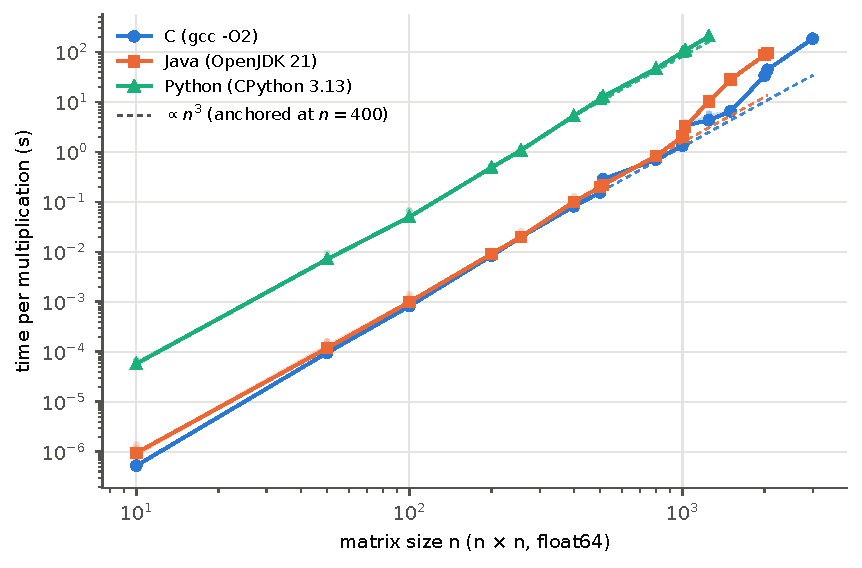
\includegraphics[width=0.86\linewidth]{../figures/fig1_runtime_loglog.pdf}
\caption{Median time per multiplication against $n$ (log--log). Bands: IQR; faint points: individual repetitions;
dashed lines: $n^3$ growth anchored at $n=400$. Python was run only up to $n=1250$ and Java up to $n=2048$ within the budget.}
\label{fig:time}
\end{figure}

\paragraph{Growth.} A least-squares fit of $\log t$ against $\log n$ gives exponents close to the cubic model only
for small to medium sizes (Table~\ref{tab:fit}): $3.17$--$3.27$ for $50\le n\le400$ in all three languages. Over the
larger windows the exponent is $3.29$ for Python, $3.63$ for C and $4.01$ for Java, i.e.\ the cost per multiply--add
is not constant. Figure~\ref{fig:norm} shows this directly: the time per multiply--add $t/n^3$ is almost flat for
Python and for C/Java up to $n\approx 1000$, and then grows (C: $1.3\to6.8$\,ns, Java: $2.0\to11.1$\,ns).
At $n=512$ and $n=1024$ C has isolated spikes (Section~\ref{sec:pow2}).

\begin{table}[H]
\centering\small
\begin{tabular}{llrrl}
\toprule
Impl. & Sizes used ($n$) & Points & Exponent $k$ & 95\,\% CI \\
\midrule
C & 50--400 & 5 & 3.27 & [3.16, 3.38] \\
C & 200--3000 & 13 & 3.63 & [3.37, 3.89] \\
Java & 50--400 & 5 & 3.22 & [3.04, 3.40] \\
Java & 200--2048 & 12 & 4.01 & [3.67, 4.36] \\
Python & 50--400 & 5 & 3.17 & [2.92, 3.43] \\
Python & 200--1250 & 9 & 3.29 & [3.19, 3.39] \\
\bottomrule
\end{tabular}

\caption{Empirical exponent $k$ in $t\propto n^{k}$ (least squares on the medians, 95\,\% $t$-interval). The interval reflects the scatter of the medians around the line, not between-process variability (Section~\ref{sec:procvar}).}
\label{tab:fit}
\end{table}

\begin{figure}[h]
\centering
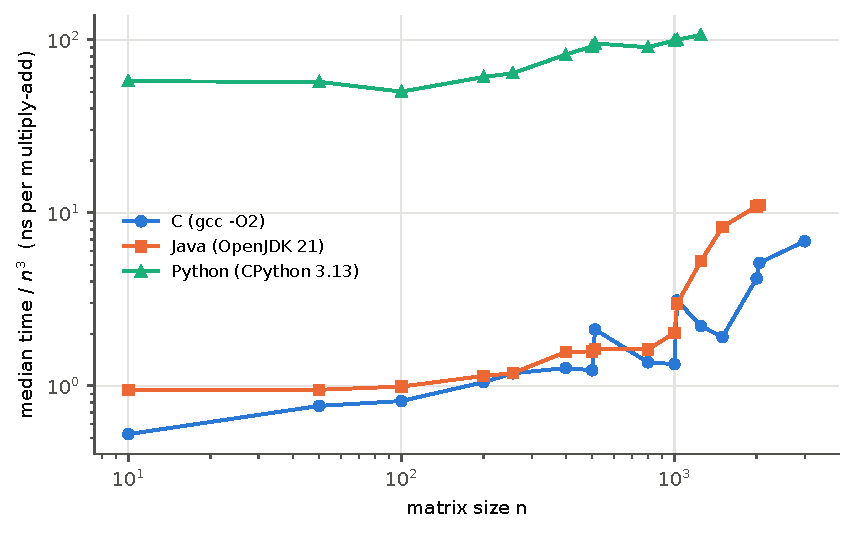
\includegraphics[width=0.82\linewidth]{../figures/fig2_normalised_time.pdf}
\caption{Median time divided by $n^3$ (nanoseconds per multiply--add). A purely cubic algorithm with constant cost per operation would give horizontal lines.}
\label{fig:norm}
\end{figure}

\paragraph{Relative speed.} For $50\le n\le1000$ Python is $54$--$75\times$ slower than C and $49$--$60\times$
slower than Java; over the whole range where both exist the Python/C ratio is $32\times$ (at $n=1024$, where C
is slow, see below) to $109\times$ ($n=10$). Java is within $0.77$--$1.51\times$ of C for $50\le n\le1024$ ($1.80\times$ at $n=10$), but
$2.4\times$ ($n=1250$), $4.3\times$ ($n=1500$), $2.6\times$ ($n=2000$) and $2.2\times$ ($n=2048$) slower at
larger sizes (\texttt{results/summary\_ratios.csv}).

\subsection{Memory}
Table~\ref{tab:mem} and Figure~\ref{fig:mem} give the peak resident memory (\texttt{VmHWM}). Memory was never the limiting
factor: the largest run (C, $n=3000$) peaked at $207.8$\,MiB, versus the $4$\,GiB budget.

\begin{table}[H]
\centering\small
\begin{tabular}{rrrr}
\toprule
$n$ & C & Java & Python \\
\midrule
10 & 1.8 & 45.7 & 9.8 \\
50 & 1.8 & 43.2 & 10.0 \\
100 & 2.0 & 43.8 & 10.9 \\
200 & 2.7 & 44.5 & 14.3 \\
256 & 3.3 & 45.0 & 17.4 \\
400 & 5.4 & 47.2 & 28.3 \\
500 & 7.5 & 49.2 & 38.7 \\
512 & 7.8 & 49.7 & 40.1 \\
800 & 16.4 & 57.6 & 83.6 \\
1000 & 24.7 & 66.5 & 125.0 \\
1024 & 25.8 & 68.0 & 130.6 \\
1250 & 37.5 & 79.3 & 189.6 \\
1500 & 53.3 & 94.9 & -- \\
2000 & 93.3 & 174.1 & -- \\
2048 & 97.8 & 174.3 & -- \\
3000 & 207.8 & -- & -- \\
\bottomrule
\end{tabular}

\caption{Peak resident memory (MiB) of the process (\texttt{VmHWM}); ``--'' where the run did not complete.}
\label{tab:mem}
\end{table}

\begin{table}[H]
\centering\small
\begin{tabular}{lrrr}
\toprule
Impl. & Baseline (MiB, $n{=}10$) & Measured bytes per $n^2$ & Model bytes per $n^2$ \\
\midrule
C & 1.8 & 24.0 & 24 \\
Java & 45.7 & 22.3 & 24 \\
Python & 9.8 & 120.9 & 120 \\
\bottomrule
\end{tabular}

\caption{Baseline (smallest run, $n=10$) and measured growth in bytes per $n^2$ (median over $n\ge500$) against the model of three
matrices ($24$ B for C/Java, $\approx120$ B for Python).}
\label{tab:membytes}
\end{table}

\begin{figure}[h]
\centering
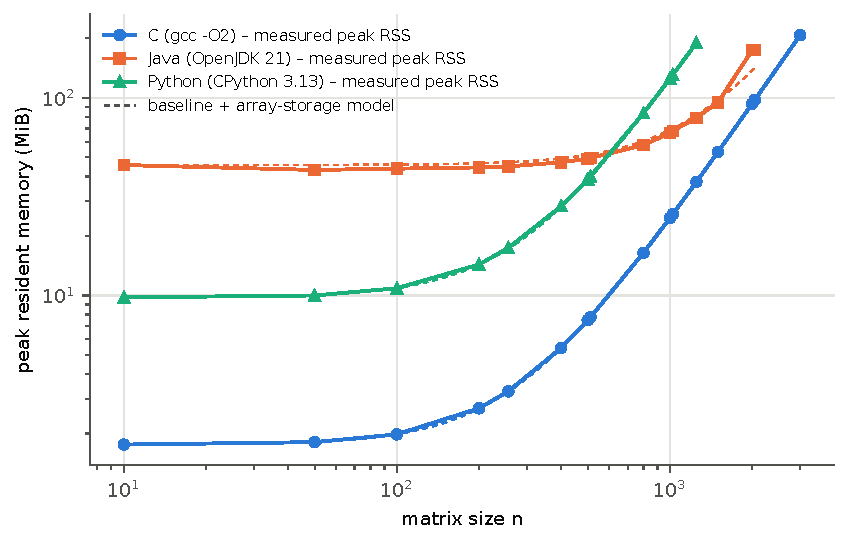
\includegraphics[width=0.82\linewidth]{../figures/fig3_memory.pdf}
\caption{Peak resident memory against $n$. Dashed lines: measured baseline of the smallest run plus the array-storage model ($24n^2$ B for C and Java, $120n^2$ B for Python).}
\label{fig:mem}
\end{figure}

C grows by $24.0$ bytes per $n^2$ (three $8$-byte matrices) on top of a $1.8$\,MiB baseline. Python grows by $120.9$ bytes
per $n^2$ ($5\times$ more) on top of $9.8$\,MiB, matching an $8$-byte pointer plus a $32$-byte float object per element
for three matrices. Java has the largest baseline ($45.7$\,MiB, the JVM itself) and grows by $\approx22$ bytes per $n^2$ up to
$n=1500$; at $n=2000$ and $2048$ it grows by $32$--$34$ bytes per $n^2$, i.e.\ about $32$\,MiB more than the three
arrays (not investigated; plausibly heap sizing by the garbage collector). The kernel's \texttt{ru\_maxrss}
(stored as a cross-check) is useless for small runs ($\approx 33$\,MiB even for C at $n=10$) because it counts the
parent driver's memory at process creation; this is why \texttt{VmHWM} was chosen as the primary metric.

\subsection{Feasible sizes and limits}
Table~\ref{tab:limits} separates the largest size that completed within the declared limits from the largest size
attempted. No run failed for memory. All failures are timeouts of a single multiplication at the $300$\,s limit; their
times are \emph{not} known, only that they exceeded $300$\,s.

\begin{table}[H]
\centering\small
\begin{tabular}{lrrl}
\toprule
Impl. & Largest feasible $n$ & Largest attempted $n$ & Outcome at largest attempted \\
\midrule
C & 3000 & 4096 & timeout ($>$300\,s per sample) \\
Java & 2048 & 3000 & timeout ($>$300\,s per sample) \\
Python & 1250 & 1500 & timeout ($>$300\,s per sample) \\
\bottomrule
\end{tabular}

\caption{Largest feasible and largest attempted size per implementation. The largest feasible size of every implementation was measured with only 2 repetitions.}
\label{tab:limits}
\end{table}

\subsection{Variability and warm-up}
Within a process, the relative IQR is mostly between $0.5$ and $20\,\%$ (Figure~\ref{fig:var}, left), with one outlier
of $36\,\%$ (C, $n=1250$); the median over all configurations is $4.8\,\%$. The first warm-up sample of Java is up to $1.3$--$1.6\times$ the steady median for some sizes
($n=50$, $400$, $500$) and about $1.0$ otherwise (right); with $3$ warm-up samples for the sizes below $1$\,s the
measured samples are in steady state. For the long runs (no warm-up) the first measured sample was within $10\,\%$ of the median (largest: $+10\,\%$, C at $n=2048$).

\begin{figure}[h]
\centering
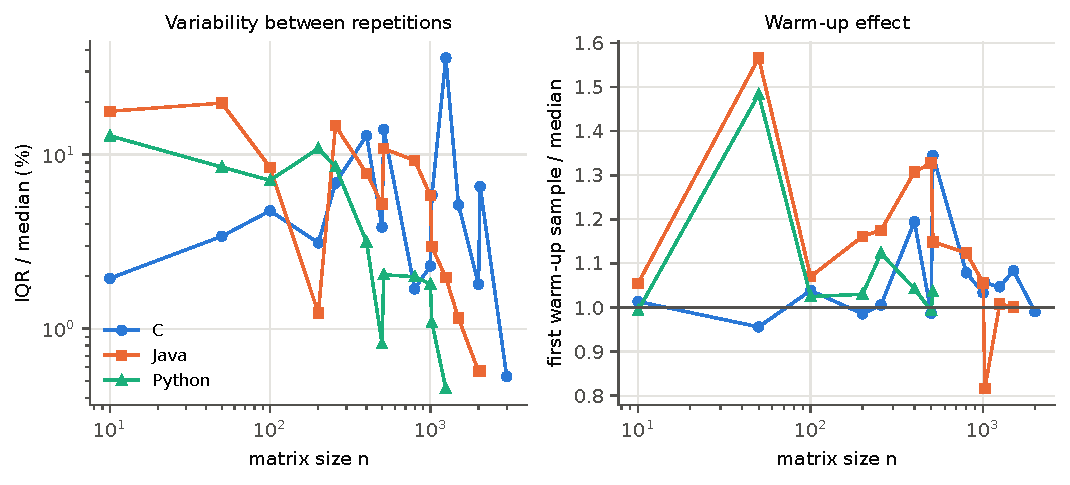
\includegraphics[width=0.95\linewidth]{../figures/fig4_variability_warmup.pdf}
\caption{Left: relative IQR of the measured samples within one process. Right: first warm-up sample divided by the median of the measured samples (only sizes with warm-up).}
\label{fig:var}
\end{figure}

\subsection{Supplementary experiments}

\paragraph{C optimisation level.}
\label{sec:cflags}
Table~\ref{tab:cflags} compares gcc optimisation levels. \texttt{-O0} is $2.2$--$3.7\times$ slower than \texttt{-O2}; \texttt{-O1},
\texttt{-O2}, \texttt{-O3} and \texttt{-O3 -march=native} are indistinguishable at $n=512$ and $n=1000$ ($\pm 6\,\%$) and differ by at
most $10\,\%$ at $n=1024$, which is within the between-process variability of Section~\ref{sec:procvar}. All variants produce the
same bits as \texttt{-O2}. The primary configuration \texttt{-O2} is therefore representative of the optimised builds for this
kernel; no vectorisation or loop interchange benefit was observed.

\begin{table}[H]
\centering\small
\begin{tabular}{lrrrc}
\toprule
Flags & $n{=}512$ & $n{=}1000$ & $n{=}1024$ & same bits as -O2 \\
\midrule
gcc -O0 & 638\,ms & 5.17\,s & 6.63\,s & yes \\
gcc -O1 & 299\,ms & 1.41\,s & 2.75\,s & yes \\
gcc -O2 & 292\,ms & 1.41\,s & 2.7\,s & yes \\
gcc -O3 & 267\,ms & 1.43\,s & 2.97\,s & yes \\
gcc -O3 -march=native & 278\,ms & 1.39\,s & 2.91\,s & yes \\
\bottomrule
\end{tabular}

\caption{C compiler options: median time per multiplication (10 repetitions at $n=512$, 5 otherwise).}
\label{tab:cflags}
\end{table}

\paragraph{Sizes around powers of two.}
\label{sec:pow2}
Table~\ref{tab:stride} and Figure~\ref{fig:pow2} show the time per multiply--add just below, at and above $2^9$ and
$2^{10}$. In C the time at $n=512$ and $n=1024$ is about $1.8$--$1.9\times$ that of the average of the neighbouring sizes
($n=512$: $2.41$ vs.\ $1.32$--$1.42$\,ns; $n=1024$: $3.04$ vs.\ $1.50$--$1.67$\,ns). The Java program with a flat array shows
the same spikes ($1.7$--$1.8\times$), whereas the Java program with \texttt{double[n][n]} shows none.

\begin{table}[H]
\centering\small
\begin{tabular}{rrrr}
\toprule
$n$ & C & Java \texttt{double[n][n]} & Java flat \texttt{double[]} \\
\midrule
496 & 1.417 & 1.631 & 1.411 \\
504 & 1.313 & 1.652 & 1.347 \\
512 & 2.410 & 1.576 & 2.325 \\
520 & 1.316 & 1.652 & 1.420 \\
1016 & 1.503 & 2.273 & 1.808 \\
1024 & 3.043 & 1.956 & 3.327 \\
1032 & 1.666 & 2.336 & 1.900 \\
\bottomrule
\end{tabular}

\caption{Median time per multiply--add (ns) around powers of two. Single process per cell.}
\label{tab:stride}
\end{table}

\begin{figure}[h]
\centering
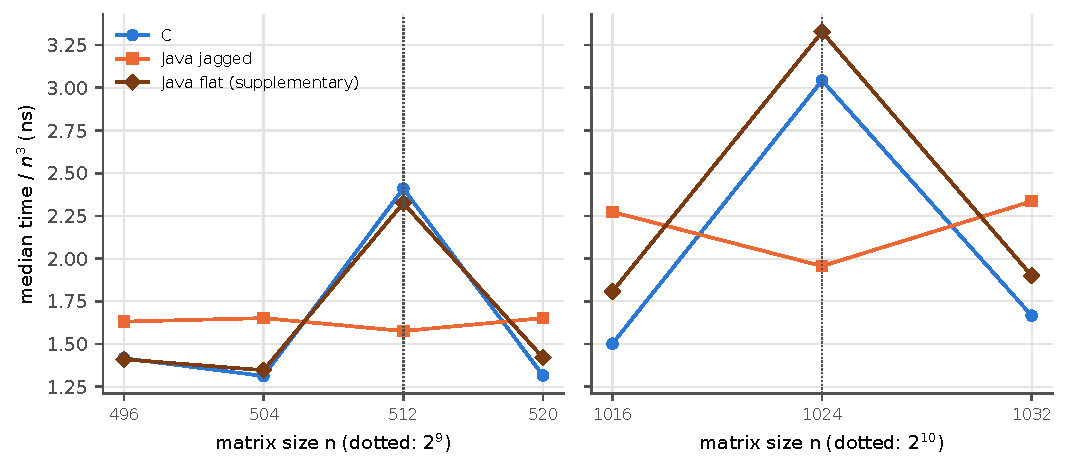
\includegraphics[width=0.92\linewidth]{../figures/fig7_powers_of_two.pdf}
\caption{Median time per multiply--add around $n=2^9$ (left) and $n=2^{10}$ (right).}
\label{fig:pow2}
\end{figure}

\paragraph{Java array layout.}
Table~\ref{tab:layout} and Figure~\ref{fig:layout} compare jagged and flat storage in Java against C. The flat
version is $1.07$--$1.49\times$ slower than C for $500\le n\le2000$, whereas the jagged version is $1.29$--$4.33\times$
slower; the jagged/flat ratio grows from $1.1$ at $n=500$--$1000$ to $1.7$--$2.9$ at $n\ge1250$. The $n=1250$ C
value has an IQR of $36\,\%$ and should be read with care.

\begin{table}[H]
\centering\small
\begin{tabular}{rrrrrr}
\toprule
$n$ & C & Java jagged & Java flat & jagged/C & flat/C \\
\midrule
500 & 154\,ms & 198\,ms & 169\,ms & 1.29 & 1.10 \\
1000 & 1.33\,s & 2.02\,s & 1.82\,s & 1.51 & 1.36 \\
1250 & 4.33\,s & 10.2\,s & 5.86\,s & 2.37 & 1.36 \\
1500 & 6.46\,s & 28\,s & 9.66\,s & 4.33 & 1.49 \\
2000 & 33.4\,s & 86.9\,s & 35.9\,s & 2.60 & 1.07 \\
\bottomrule
\end{tabular}

\caption{Median time per multiplication for C, Java with \texttt{double[n][n]} (jagged), and Java with a flat \texttt{double[]} (supplementary), and ratios.}
\label{tab:layout}
\end{table}

\begin{figure}[h]
\centering
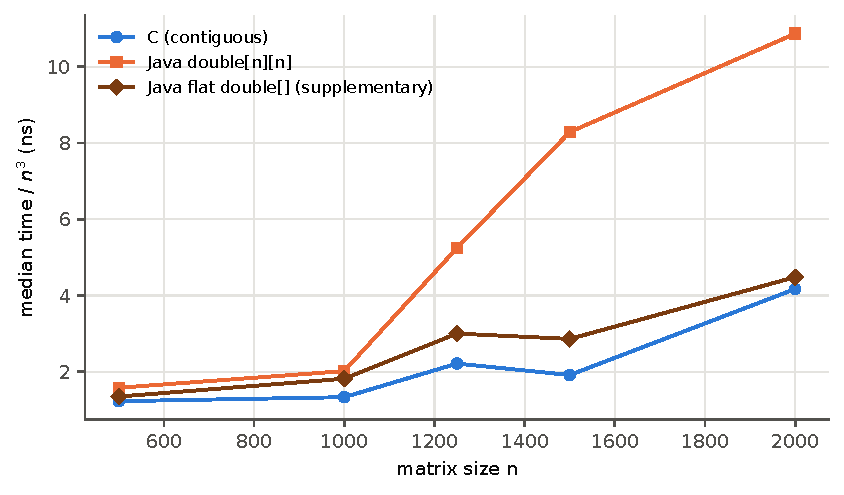
\includegraphics[width=0.82\linewidth]{../figures/fig8_java_layout.pdf}
\caption{Time per multiply--add for C and the two Java layouts.}
\label{fig:layout}
\end{figure}

\paragraph{Between-process variability.}
\label{sec:procvar}
Table~\ref{tab:procvar} reports the median time at $n=1024$ in six independent processes. For C the six medians
span $13\,\%$ of their median ($2.96$--$3.38$\,s), for Java $40\,\%$ ($2.10$--$3.21$\,s). Within each process the relative IQR
is $2$--$12\,\%$ for C and $3$--$28\,\%$ for Java (the min--max range of Java reaches $47\,\%$ of the median), so at this size the
timing is noisy both within and between processes. A single-process median at $n=1024$ is therefore uncertain by tens of
percent for Java, and differences of that size between C and Java at this $n$ cannot be resolved.

\begin{table}[H]
\centering\small
\begin{tabular}{lrr}
\toprule
Independent process & C & Java \\
\midrule
1 & 3.34\,s & 3.21\,s \\
2 & 3.27\,s & 2.1\,s \\
3 & 3.06\,s & 2.44\,s \\
4 & 2.96\,s & 2.75\,s \\
5 & 3.35\,s & 2.77\,s \\
6 & 3.38\,s & 3.08\,s \\
\textit{min} & 2.96\,s & 2.1\,s \\
\textit{median} & 3.3\,s & 2.76\,s \\
\textit{max} & 3.38\,s & 3.21\,s \\
range / median & 13\,\% & 40\,\% \\
\bottomrule
\end{tabular}

\caption{Median time per multiplication at $n=1024$ in six independent processes (process 1 is the main run).}
\label{tab:procvar}
\end{table}

\section{Discussion}

\subsection{Answer to the research question}
In this environment, the time of the basic $O(n^3)$ multiplication grows close to cubically for small and medium
matrices ($k\approx3.2$ for $50\le n\le400$ in all three languages), but the cost per multiply--add \emph{increases}
for larger matrices in the compiled/JIT languages: in C from $1.0$--$1.4$\,ns ($200\le n\le1000$, excluding $n=512$) to $6.8$\,ns
($n=3000$), in Java from $\approx1.6$\,ns to $11.1$\,ns ($n=2048$); in Python it rises from $50$--$60$\,ns to
$\approx100$\,ns. Python is $49$--$75$ times slower than C and Java at $50\le n\le1000$. C and Java are
comparable for $50\le n\lesssim1000$ (ratio $0.77$--$1.51$), after which the \texttt{double[n][n]} Java program falls behind
($2.2$--$4.3\times$). Memory is explained by array storage plus a runtime baseline: $24$, $\approx22$ (Java, $n\le1500$) and
$\approx121$ bytes per $n^2$, with baselines of $1.8$, $45.7$ and $9.8$\,MiB for C, Java and Python. Time, not memory, limits
the feasible size: $n=3000$ (C), $2048$ (Java), $1250$ (Python) under a $300$\,s-per-multiplication limit.

\subsection{Hypotheses}
\begin{itemize}
  \item \textbf{H1 (cubic growth)}: supported only partially. The exponent is $3.17$--$3.27$ for $n\le400$, but $3.29$ (Python),
        $3.63$ (C) and $4.01$ (Java) over the larger windows. The operation count is cubic; the \emph{time} is not, because the cost
        per operation depends on $n$ (Figure~\ref{fig:norm}).
  \item \textbf{H2 (C $\lesssim$ Java $\ll$ Python)}: Python is $49$--$75\times$ slower for $50\le n\le1000$, consistent with ``one to two orders
        of magnitude''. C $\lesssim$ Java holds only for $50\le n\lesssim1000$ (within noise); beyond that Java is up to $4.3\times$ slower.
  \item \textbf{H3 (cost per operation rises with $n$)}: supported in all three languages (C $0.5\to6.8$\,ns, Java $0.9\to11.1$\,ns,
        Python $50\to106$\,ns), with additional spikes at powers of two.
  \item \textbf{H4 (memory model)}: supported for C ($24.0$ B$/n^2$) and Python ($120.9$ B$/n^2$); Java matches ($22.3$) up to $n=1500$ but
        needs $\approx32$ B$/n^2$ at $n\ge2000$.
\end{itemize}

\subsection{Interpretation, and how strong the evidence is}
\paragraph{Python.} The $\approx50$--$60$\,ns per multiply--add for $n\le200$ is the cost of executing the inner loop in the
interpreter, where each iteration performs several bytecode dispatches, two double indexings and the allocation of a float object;
this is consistent with the observed constant per-operation cost at small $n$ and the $\approx50$--$75\times$ gap, but the cost
of individual bytecodes was not measured here. The further increase to $82$--$106$\,ns at $n\ge400$ coincides with the working set
growing beyond the caches (about $40$ bytes per element, Table~\ref{tab:mem}), where every access dereferences a pointer to a float
object; Python's increase ($\approx2\times$) is smaller than in C ($\approx5\times$) because interpreter overhead is a large constant part of its cost.

\paragraph{C: powers of two and large $n$.} Two effects are visible. (i) At $n=512$ and $1024$ the matrix row stride is a multiple of
$4096$ bytes, so the successive elements $b_{kj}$ of a column are mapped to few cache sets; the time per multiply--add jumps by
$\approx1.8$--$1.9\times$ relative to $n\pm$ a few (Figure~\ref{fig:pow2}). The effect appears in C and in Java with a flat array,
and not in Java with \texttt{double[n][n]}, which is consistent with a memory-layout explanation (row addresses of separately allocated
Java arrays are not exact multiples of the page size) \cite{drepper,hennessy}. (ii) For $n\gtrsim1250$ the cost per operation grows
steadily (Figure~\ref{fig:norm}). The matrix $B$ occupies $8n^2$ bytes ($8$\,MB at $n=1000$, $32$\,MB at $n=2048$, $72$\,MB at $n=3000$),
which exceeds the L2 cache ($2$\,MiB per core) and approaches or exceeds the L3 cache ($33$\,MiB, shared) of this machine, and a column
walk touches a different $4$\,KiB page at every step for $n\ge512$, which also stresses the address-translation caches. These are plausible
causes, consistent with the trend, but \textbf{they were not measured}: no hardware performance counters were available in the virtual
machine, so cache misses and TLB misses were not observed.

\paragraph{Java versus C.} The gap in Figure~\ref{fig:time} is not a property of the JIT arithmetic: Java with a flat array is within
$1.07$--$1.49\times$ of C for $500\le n\le2000$, whereas the \texttt{double[n][n]} version is up to $4.3\times$ slower, and the
jagged/flat ratio grows with $n$. A jagged array adds, for every $b[k][j]$, a load of the row reference and a length check on a
\emph{separate} object, and rows are separate memory blocks; at large $n$ this plausibly increases cache and TLB pressure. The experiment
supports ``layout explains most of the gap'' but does not identify the mechanism, and the remaining $7$--$49\,\%$ (bounds checks,
JIT code quality, or other effects) was not isolated. Warm-up played a minor role: the first warm-up sample was at most $1.6\times$ the steady
value and the measured samples were stable (Figure~\ref{fig:var}).

\paragraph{C compiler options.} \texttt{-O0} is $2.2$--$3.7\times$ slower; \texttt{-O1} to \texttt{-O3} are indistinguishable within the noise.
Because floating-point reductions cannot be re-associated without \texttt{-ffast-math} and the column access of $B$ is strided, the
compiler has little to improve; \texttt{-march=native} did not help either. This supports using \texttt{-O2} as a representative optimised
configuration for this particular kernel, nothing more.

\subsection{Limitations}
\begin{itemize}
  \item \textbf{One virtual machine.} All data come from one $2$-vCPU KVM guest on a shared host: other tenants, frequency scaling and
        host scheduling are not observable or controlled, and the processes were not pinned. Absolute times are not transferable to other machines.
  \item \textbf{Between-process variability.} At $n=1024$ the median of six independent processes varies by $13\,\%$ (C) and $40\,\%$ (Java)
        and the within-process spread of Java is also large. Most comparisons of ratios close to $1$ at a single size (e.g.\ Java/C
        $=0.77$ at $n=512$ or $0.96$ at $n=1024$) are therefore \emph{not} significant. The IQRs in Table~\ref{tab:time} describe
        within-process repetitions only.
  \item \textbf{Few repetitions at large $n$} (2--3, forced by the budget), a single pair of input matrices per size, and a single run
        order per size (interleaved by language to reduce, not eliminate, time-of-day effects).
  \item \textbf{Exploratory supplementary experiments.} They were designed after seeing the main results, have one process per cell (except $n=1024$) and
        test explanations indirectly; the mechanisms above remain hypotheses.
  \item \textbf{Scope.} Results apply to gcc $13.3$ \texttt{-O2}, OpenJDK $21$ with the serial GC, CPython $3.13$ and the algorithm, layouts and
        inputs described here. They do not support a statement that one language is faster than another in general; other compilers, JVM settings, Python
        implementations or matrix libraries could change the picture drastically (and are the topic of the next assignments).
  \item \textbf{Memory metric.} RSS is not the same as heap use or allocated storage; the Java excess at $n\ge2000$ was not investigated.
\end{itemize}

\section{Conclusions}
\begin{enumerate}
  \item Under the described conditions, the basic triple-loop multiplication takes $\approx n^{3.2}$ for $n\le400$ in C, Java and
        Python, and the cost per multiply--add rises for larger matrices (C up to $6.8$\,ns at $n=3000$, Java $11.1$\,ns at
        $n=2048$, Python $\approx100$\,ns at $n\approx1000$--$1250$).
  \item Python is $49$--$75\times$ slower than C and Java for $50\le n\le1000$. C and Java agree within a factor of $1.5$ for $50\le n\lesssim1000$;
        beyond, \texttt{double[n][n]} Java is $2.2$--$4.3\times$ slower than C, and a flat-array Java variant removes most of that gap ($\le1.5\times$ of C).
  \item C (and flat Java) is $\approx1.7$--$1.9\times$ slower at $n=512$ and $n=1024$ than at neighbouring sizes.
  \item Memory follows array storage plus a runtime baseline: $24$ B$/n^2$ (C), $\approx22$ (Java, $n\le1500$), $\approx121$ (Python), with baselines $1.8$, $45.7$ and $9.8$\,MiB.
  \item With a $300$\,s per-multiplication limit the largest feasible sizes were $3000$ (C), $2048$ (Java) and $1250$ (Python); the first
        failures ($4096$, $3000$, $1500$) were timeouts, never memory failures.
  \item Unresolved: the hardware mechanisms behind the large-$n$ slowdown and the power-of-two spikes (needs performance counters),
        the origin of Java's extra memory at $n\ge2000$, and the effect of the machine (needs repetition on other hardware).
\end{enumerate}
The numbers apply to this experiment only; the optimisation techniques that address several of the observed effects (loop order, blocking, sparse
formats) are left for Assignment~2.

\section{Use of generative AI}
In line with the course policy, the use of AI is disclosed: the tool was \textbf{Claude (Anthropic)}. It was used for planning the experimental
design, writing the benchmark driver, the test and analysis scripts, the supplementary experiments and a first draft of this report.
The affected parts are \texttt{scripts/}, \texttt{src/} and \texttt{report/}. The author is responsible for understanding the code, validating the measurements,
checking the references and defending the conclusions; generated text is not evidence, and every number in this report was produced by the included code
from the raw data in \texttt{results/}.

\section{Reproducibility materials}
\label{sec:materials}
Source code, build and run instructions, raw measurements, input-generation scripts and analysis scripts are in the repository
\repourl{} and in \path{Assignment01_GonzalezFernandez_Materials.zip}. The \texttt{README.md} gives the exact commands
(\texttt{make build inputs test bench cflags analyze report}); the input matrices are not stored but regenerated with
\texttt{scripts/gen\_inputs.py} and verified against the SHA-256 digests in \texttt{data/manifest.json}. Raw data:
\path{results/raw_measurements.csv} (one row per sample, warm-up included) and \path{results/runs.csv} (one row per process);
environment: \path{results/environment.json}; every figure and table is generated by \path{scripts/analyze.py}.
The basic triple-loop structure was taken from the example implementations (Python, Java, Rust and C, $1024\times1024$) that were given to the author as examples for this
assignment; their timings were not used. The shared binary inputs, the scalar-accumulator kernels, monotonic timers, measurement driver, validation, supplementary experiments and analysis were
written for this study with the AI assistance disclosed above. No other external code, text or figures are reused. All numbers in this report come from the run documented in
\texttt{results/}.

\begin{thebibliography}{99}
\bibitem{clrs} T.~H.~Cormen, C.~E.~Leiserson, R.~L.~Rivest and C.~Stein, \emph{Introduction to Algorithms}, 4th~ed. Cambridge, MA, USA: MIT Press, 2022.
\bibitem{drepper} U.~Drepper, ``What every programmer should know about memory,'' Red~Hat, Inc., Nov. 2007.
\bibitem{hennessy} J.~L.~Hennessy and D.~A.~Patterson, \emph{Computer Architecture: A Quantitative Approach}, 6th~ed. Cambridge, MA, USA: Morgan Kaufmann, 2017.
\bibitem{higham} N.~J.~Higham, \emph{Accuracy and Stability of Numerical Algorithms}, 2nd~ed. Philadelphia, PA, USA: SIAM, 2002.
\bibitem{goldberg} D.~Goldberg, ``What every computer scientist should know about floating-point arithmetic,'' \emph{ACM Comput. Surv.}, vol.~23, no.~1, pp.~5--48, Mar. 1991.
\bibitem{georges} A.~Georges, D.~Buytaert and L.~Eeckhout, ``Statistically rigorous Java performance evaluation,'' in \emph{Proc. 22nd ACM SIGPLAN Conf. Object-Oriented Programming Systems, Languages and Applications (OOPSLA)}, Montreal, Canada, 2007, pp.~57--76.
\bibitem{hoefler} T.~Hoefler and R.~Belli, ``Scientific benchmarking of parallel computing systems: Twelve ways to tell the masses when reporting performance results,'' in \emph{Proc. Int. Conf. High Performance Computing, Networking, Storage and Analysis (SC '15)}, Austin, TX, USA, 2015, Art.~no.~73.
\bibitem{numpy} C.~R.~Harris \emph{et al.}, ``Array programming with NumPy,'' \emph{Nature}, vol.~585, pp.~357--362, 2020, doi: 10.1038/s41586-020-2649-2.
\bibitem{py312} Python Software Foundation, ``What's new in Python 3.12,'' Python documentation (built-in \texttt{sum()} uses compensated summation for floats; CPython issue gh-100425).
\end{thebibliography}


\end{document}
